%floatsintext can be used in man to have figs appear where they are called
\documentclass[man, noextraspace, apacite, floatsintext]{apa6}
%following looks like a journal printout; need to comment out previous line
%\documentclass[jou,noextraspace,apacite]{apa6}
\usepackage{apacite}
\usepackage{setspace}
\usepackage{listings}
\lstset{
basicstyle=\small\ttfamily,
columns=flexible,
breaklines=true
}

\title{Use Welch's \textit{t} test to Compare the Means of Independent Groups}
\shorttitle{Welch t Test}

\twoauthors{Joshua D. Wondra}{Richard Gonzalez}
\twoaffiliations{Facebook}{University of Michigan}

\abstract{Researchers typically use Student's t test or ANOVA to test whether the means of independent groups are different from each other.  
These tests assume that the population variances of the groups are equal. If there is 
reason to believe the variances are unequal, then researchers can 
use Welch's t test, which does not assume equal variances, as an alternative. 
We were interested in finding a simple rule to 
decide when to use Student's vs. Welch's t test. We used Monte Carlo 
simulations to compare the false positive rate, power, and coverage probability 
of Student's and Welch's t tests across different variance ratios, sample size ratios, sample sizes, 
and effect sizes. We examined a simple case---the difference in the means of 
two groups---and a more complex case---the test of the interaction in a 
2~$\times$~2 factorial design. We recommend the following rule: 
If the data are normally distributed, always use Welch's t test to 
compare the means of independent groups.}
\keywords{Welch t test, contrasts, hypothesis testing, simulation}

\authornote{Joshua D. Wondra, Facebook.

Richard Gonzalez, Department of Psychology, University of Michigan.

This research was conducted while Josh Wondra was a graduate student at the University of Michigan.

Correspondence concerning this article should be addressed to Josh Wondra, 
Facebook, 770 Broadway, New York, NY, 10003.

Contact: jdwondra@umich.edu}


\usepackage{Sweave}
\begin{document}
\Sconcordance{concordance:WelchManuscript-MASTER.tex:WelchManuscript-MASTER.Rnw:%
1 66 1 48 0 1 85 7 1 1 16 10 1 1 16 14 1 1 20 10 1 1 4 10 1 1 4 9 %
1 1 69 9 1 2 0 11 1 2 0 4 1 1 150 1 1 1 152 11 1 1 8 6 1 1 122 2 1 %
1 122 6 1 1 0 12 1 1 7 4 1 1 225 5 1}

\maketitle
    Data analysis involves decisions about which statistical test answers the research question, whether the test is 
suitable to the data, and whether there is a more appropriate test. Recent discussions of research practices in psychology 
\cite<e.g.,>{Fiedler2012, Simmons2011, 
Wagenmakers2012} highlight the tension between two valued outcomes of these 
decisions. On the one hand, researchers don't want to mistakenly 
claim there is a true effect where none exists, which involves a 
concern with false positives. On the other hand, researchers want to find 
effects where they do exist, which involves a concern with power. In addition,
there is a growing concern with estimating effect sizes 
\cite{Bakker2012, Cumming2014, Ioannidis2008}. 
Researchers must find a way to balance these concerns as they make their decisions. 

The recent push for pre-registration forces researchers to make these decisions prior to data collection by specifying how they plan to test their hypothesis (e.g., a two-sample t test). But they should also address the assumptions of those tests (e.g., equal variances), how they will check if those assumptions are violated (e.g., a significance test of two variances), and what they will do in that case (e.g., use a different test).  Such planning can be good for science, but it can easily become overwhelming to write a long list of conditional statements: ``if I see this, then I'll do that.''  Preregistration can be simplified if the researcher commits to a statistical procedure that is robust to violations of assumptions, and all the better if the procedure doesn't introduce new costs, such as lower power. We propose that when researchers compare the means of independent groups, they should commit to Welch's t test, which is robust when variances are unequal, instead of Student's t test or ANOVA. 

\subsection{The Comparison of Means from Independent Groups}
    One of the first decisions many researchers learn is how to compare 
the means of two independent groups---they run a t test. But even this basic 
comparison involves a choice between the classic Student's t test 
\cite{Student1908} or the alternative Welch-Satterthwaite test \cite{Welch1938, 
Satterthwaite1946}. When you use Student's t test to compare 
the means of independent groups, you assume the populations follow a normal distribution,
observations are independent of each other, and the populations have the same variance. Throughout the paper we assume that the null hypothesis of for the population mean difference is zero.
    
The t-value is the 
difference in group means divided by the standard error of that 
difference:   
    \begin{equation}
    t = \frac{\hat{\mu}_1-\hat{\mu}_2}{\hat{\sigma}_{\mu_1-\mu_2}}
    \end{equation}
The p-value also depends on the degrees of 
freedom, $df=n_1+n_2-2$. You are more likely to reject the null 
hypothesis
as the t-value and 
degrees of freedom get larger---when 
the sample size gets larger (which increases the degrees of freedom and influences the standard error), when the 
difference in means gets larger (which increases the numerator of t), or 
when the standard error gets smaller (which decreases the denominator of t). 
    
    To compute the usual standard error, you need to find the 
common variance of the groups. If the the equal variances assumption is true, then the common variance is
equal to the population variance of either group.
In practice, you rarely know the population variances of the groups, so you estimate them from the sample variances. 
But even if the population variances are equal, typically the sample 
variances are not, due to sampling error. Student's t test deals with this
problem by pooling the sample variances into a weighted 
average to estimate the common variance. 
    \begin{equation}
    s_p^2 = \frac{(n_1 - 1)s_1^2 + (n_2 - 1)s_2^2}{n_1 + n_2 - 2}
    \end{equation}
    \begin{equation}
    s_{\overline{x}_1-\overline{x}_2} = \sqrt{\frac{s_p^2}{n_1}  + \frac{s_p^2}{n_2}} = s_p\sqrt{\frac{1}{n_1}  + \frac{1}{n_2}}
    \end{equation}
    with $s_1^2$ and $s_2^2$ being the two sample variances.
In the pooling equation (EQ 2), if the sample sizes are different, the variance of the group 
with the larger sample size is given more weight. If the larger group has the larger 
variance, then the standard error will be larger; if the larger group has the smaller variance, then the standard error will be smaller.

    If the data or study design suggests the assumptions of 
normality, independence, and equal variances do not hold, then Student's t test 
is not the right choice. If the group 
variances are unequal, then the Welch-Satterthwaite t test (Welch's t test for the sake of brevity) is a good alternative.  In SPSS, Welch's t test is in the ``Equal 
variances not assumed'' row when you run an independent samples t 
test. In R, it's the default when you use the
\texttt{t.test()} function, and you can get Student's t test by setting 
the \texttt{var.equal} argument to \texttt{TRUE}.
    
        Like Student's t test, Welch's t test assumes normality and 
independence; however, it does not assume equal variances. The standard error is based on separate group variances instead of a 
common variance:
    \begin{equation}
    s_{\overline{x}_1-\overline{x}_2} = \sqrt{\frac{s_1^2}{n_1} + \frac{s_2^2}{n_2}}
    \end{equation}
Additionally, Welch's t test uses a complicated formula to compute the degrees of freedom: 
    \begin{equation}
    df = \frac{(\frac{s_1^2}{n_1} + \frac{s_2^2}{n_2})^2}{\frac{(s_1^2)^2}{n_1^2(n_1-1)} + \frac{(s_2^2)^2}{n_2^2(n_2-1)}}
    \end{equation}
The important thing to know is the formula decreases the degrees of freedom to the extent that the group
variances differ. It can also produce a degrees of freedom value that is not an integer.

Due to these differences in the standard errors and degrees of freedom, Student's and Welch's t tests can disagree about whether the group means are different. Because Welch's t test decreases the degrees of freedom, it might be more conservative. Welch's t test might be the better choice if it finds fewer false positives when the variances are unequal. But it might be the worse choice if it's too conservative and isn't powerful enough to detect true effects. 
        
    However, Welch's t test might not always be more conservative. The power of 
the two tests is based on not only the degrees of freedom, but also the 
standard error.  Welch's t test could be more powerful than 
Student's when its standard error is smaller.
    
    How do you decide which test to use? The typical approach is to use 
Student's t test unless you have evidence that the variances are unequal. The challenge is how to find that evidence. 
Our goal is to find a simple strategy to decide which test to use. We discuss two decision strategies in the main text---using a statistical test of the equal variances assumption and visually examining the data with boxplots---and one decision strategy in the supplemental materials---comparing the degrees of freedom of the two tests. Then we use Monte Carlo simulations to empirically determine when each test performs best.

    Before we proceed, we note that aside from Welch's t test, there have been Bayesian approaches 
to comparing groups with equal or unequal variances \cite{Box1973, Kruschke2013}. Our purpose is to inform decisions about how to use 
frequentist approaches, so we do not discuss
Bayesian approaches further.

\subsection{Testing Assumptions with Another Test}
    One way to decide which test to use
is to run another test of the null hypothesis that the group variances 
are equal. If the test retains the null, the variances are equal and you can use Student's t test. If the test rejects the null, the variances are unequal and you should use Welch's t test.

One example of this approach is Levene's test for homogeneity \cite{Levene1960}, which appears in SPSS by default when you run an independent samples t test.
In its original formulation, the test finds how far each observation deviates from the mean of its group, then it uses ANOVA to test whether the average deviations are different between the groups (later formulations use deviations from the group median or the trimmed mean, which work better when the raw data are not normally distributed, \citeNP{Brown1974}).

Consider the logic of using Levene's test to decide whether to use Student's or Welch's t 
test. You use an ANOVA to test 
whether the deviations from the group means are different.
When there are only two groups, this is equivalent to using a t test, which means you have to make another choice
between Student and Welch, which means you must decide whether the
group \textit{deviations} have equal variances.
This doesn't solve the original problem, it just hides it in a different test. 

Additionally, tests of assumptions,
like other tests, are sensitive 
to sample size \cite{Gonzalez2008}. If your sample is too small, you won't have enough power to 
detect true differences in the variances. If your sample is very 
large, even minute differences will be statistically significant. 

Overall, using tests of equal variances is an ineffective decision strategy \cite{Zimmerman1996,Zimmerman2004}. 

\subsection{Visualizing Data with Boxplots} 

    A second way to decide which test to use is to visualize the data using boxplots and judge 
whether the variances appear to differ.  With smaller samples, you 
can tolerate larger apparent differences and still conclude the variances are equal. You can enhance this strategy by 
simulating data that have the same sample sizes as the real data, changing whether the variances are equal or not, 
and checking if the boxplots from the real data look more like the boxplots of 
simulations with equal variances or unequal variances. 

    Figure 1 displays sample boxplots where two groups have equal 
variances (top) and where one group has five times the variance of the other (bottom), and where each group has $n$ = 20 (first rows) or $n$ = 
100 (second rows). 

  With smaller 
sample sizes it's typical to see 
variability in the spread of the groups. When the population 
variances are equal,
sometimes the spread of the groups appears almost equal (as it should), 
and other times it appears to differ. When the population variances are unequal, the group with the larger variance (to the right) is generally more spread out, but sometimes the spread of the groups looks similar.

In contrast, with larger sample sizes there is more 
consistency in the boxplots. Smaller differences in the spread of the groups 
might be a sign that the population variances differ. Using boxplots
to decide which test to use
is a viable strategy, though it requires some subjective judgment,
especially when sample sizes are small.

   
\begin{figure}[!ht]
\includegraphics{WelchManuscript-MASTER-boxplots}

\textit{Figure 1.} Boxplots from simulations of groups with equal variances (top) and unequal 
variances (bottom).
\end{figure}

\subsection{When Does Each Test Perform Best?}

    So far, we have been following the standard procedure---use Student's t test 
by default and  switch to Welch's t test if the variances 
are unequal. However, this approach might be
unwarranted. When the variances and sample sizes are equal, the two tests are equivalent. If Welch's t test generally comes to similar or better 
decisions than Student's, whether the variances and sample sizes are equal or not, then 
it would be better to always use 
Welch's t test. 

To investigate this possibility, we ran simulations of two independent groups 
with normally distributed data.  But the use of t tests can also be expanded to study designs with more than two groups, where they can be used to test main effects, interactions, or other specific contrasts. So we also examined the more complex case of a 2~$\times$~2 between-subjects design with a crossover interaction but no main effects.

We examined how well each test balances concerns with 
false positives, power, and effect size estimation under 
different variance ratios, sample sizes, sample size ratios, and effect sizes. 
For the 2~$\times$~2 design we varied the variance and sample size of just one group. 
Sample size did not affect the comparative performance of the two tests, so in the main text we only show cases where the smallest sample was 50. The supplemental materials have cases where the smallest sample was 20 or 100 as well.  
Some prior research has examined the 
false positive rate \cite{Boneau1960, Zimmerman1993, 
Zimmerman2004, Zimmerman1996, Zimmerman2009} and
power of the two tests when comparing two groups \cite{Neuhauser2002, 
Zimmerman1993}, though not with the complete configuration of 
conditions that we examined. Nevertheless, it will be informative to display 
the false positives and power of the two tests here. We also discuss 
implications for estimating effect sizes, which follows from the false positive
results but has not, to our knowledge, been discussed explicitly in past 
research.

    
\subsubsection{False Positive Rates}

    The expected false positive rate is $\alpha = .05$. The observed false positive 
rate for Student's t test remained close to the expected rate when either 
the population variances or sample sizes were equal, but it varied widely 
when both the variances and sample sizes were unequal (see Figure 2). 
When the larger group(s) had the larger variance, the false positive rate dropped as low as 
about .01, but when it had the smaller 
variance, the false positive rate 
rose as high as .13, more than double the expected rate. 
In contrast, the observed false positive rate for Welch's t test 
remained close to the expected rate across all conditions. Overall, Welch's 
t test consistently behaved as expected when it came to false positives. 
Student's t test did not.


\begin{figure}[!ht]  

\includegraphics{WelchManuscript-MASTER-FalsePositivePlots}

\textit{Figure 2.} False positive rates for Student's t test and Welch's t test 
as the variance ratio, sample size ratio, and sample sizes vary.
\end{figure}


\subsubsection{Power}



\begin{figure}[!ht]
\includegraphics{WelchManuscript-MASTER-PowerPlots}

\textit{Figure 3.} Power of Student's and Welch's t tests to detect a medium effect.
\end{figure}

    Is Welch's t test underpowered compared to Student's t test? Figure 3 
displays the power of the two tests to detect a medium (d = .5) effect
under the different conditions, as well as the difference in power, with higher numbers meaning that Student's t test is more poweful (results for small and large effect sizes are available in the supplemental materials). For both tests, power decreased as variances 
became unequal because we increased one or more groups' variances; however, 
it decreased at different rates depending on the sample size and 
variance ratios. When the sample sizes or variances were equal, power was approximately equal. However, when both the sample sizes and 
variances were unequal, there were differences. Student's t 
test was more powerful when the large sample(s) had the smaller variance, whereas 
Welch's t test was more powerful when the small sample(s) had the smaller variance. 
    
    Student's t test had the greatest power over 
Welch's when one sample size was twice the other and the large 
group(s) had the small variance. These are the same conditions where Student's t 
test more than doubled the expected false positive rate. So the advantage of Student's t test
in power is undermined by its inflated false 
positive rate. In contrast, Welch's t test was more 
powerful when the small group had the smaller variance, but it never inflated the false positive rate. 
These joint results, on the false positive rate and power, support the decision to always use Welch's t test. By using 
Welch's t test, you sometimes have greater power to detect true effects, but 
you don't have to worry about sacrificing concerns with false positives.  


\subsubsection{Coverage Probability}
We used 95\% confidence intervals constructed using Student's and Welch's t 
tests to find their relative coverage probability, the proportion of confidence intervals 
that contain the population value of the estimated parameter, which in this case is the 
difference in group means. By 
definition,  the expected coverage probability of 95\% confidence intervals  is .95. 
% Because the coverage 
% probability of a confidence interval is not influenced by the effect size, we 
% only show the coverage probabilities when the null hypothesis is true. 
Additionally, when the null hypothesis is true and $\alpha = .05$, the coverage 
probability of 95\% confidence intervals has a simple relationship with the 
false positive rate---it's the complement of the false positive rate. 

Figure 4 displays the coverage probabilities of the two t tests. 
The coverage probability for Student's t test varies dramatically, just as the 
false positive rate did.  When Student's t test is the most 
powerful, it is also the least accurate at estimating the difference in means, and what you would believe is a 95\% 
confidence interval drops to as low as an 87\% confidence interval in reality. 
In contrast, Welch's t test performs as expected and the confidence interval 
contains the true effect 95\% of the time regardless of the variance and sample 
size ratios. 


\begin{figure}[!ht]
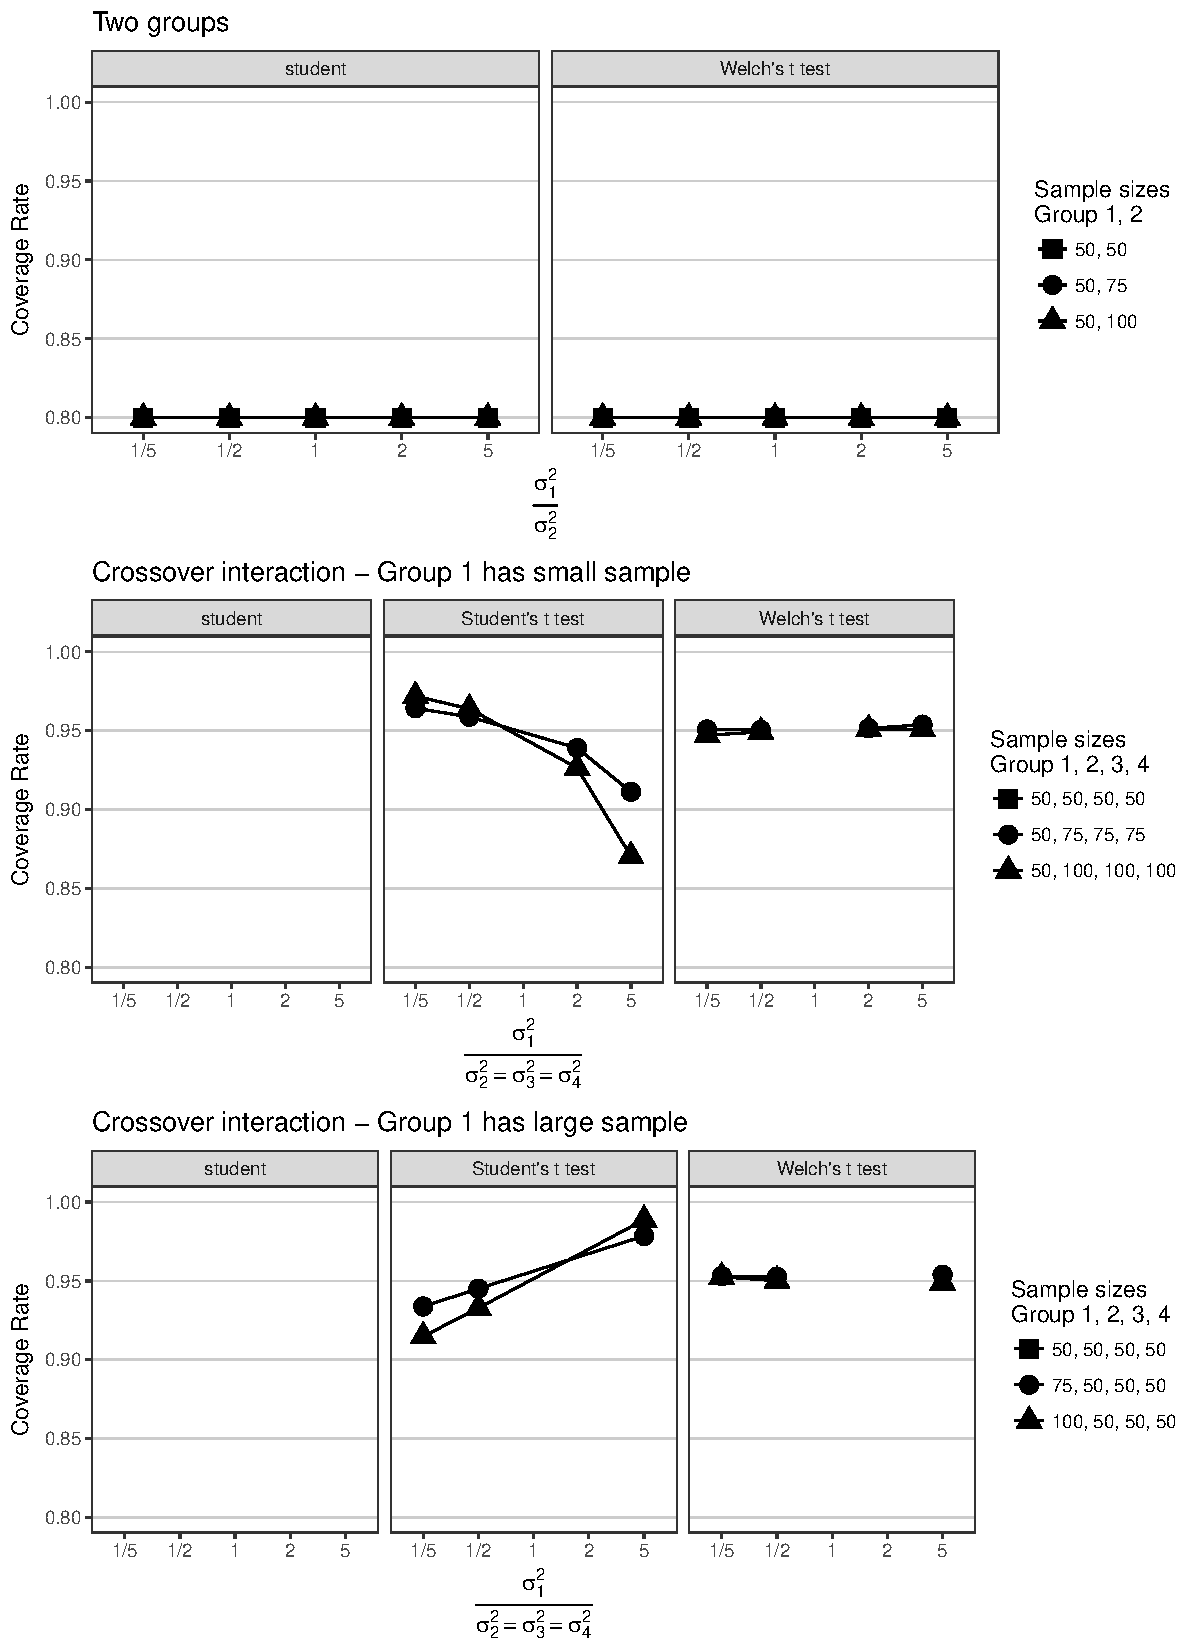
\includegraphics{WelchManuscript-MASTER-CoveragePlots}

\textit{Figure 6.} Coverage probabilities for Student's and Welch's t tests.
\end{figure}




\section{Discussion}
    We set out to find a simple rule to help researchers decide when to use 
Student's t or Welch's t test. We believe the simplest 
rule is to always use Welch's t test to compare the means of independent groups, whether there are two groups or more.
    
    The simulations demonstrated that when the population 
variances or sample sizes were equal, using Welch's t test instead of Student's 
didn't hurt. Though the degrees of freedom from Welch's t test can 
drop substantially below Student's when only the variances 
or only the sample sizes are unequal (see Figure S1), the simulated false positive rates, 
power, and coverage probabilities were almost identical under 
these conditions. The difference in the degrees of freedom had a 
negligible effect on the outcomes. 
    
    More important was the standard error, which 
affects the t-value. When either the variances or sample sizes are 
equal, the pooled standard error of Student's t test and the separate variances 
standard error of Welch's t test are identical, and the two tests will 
generally agree with each other. However, when both the variances and the 
sample sizes are unequal, the pooled standard error of Student's t test gives 
more weight to the larger group \cite<e.g.,>{Coombs1996,Zimmerman2009}; if that group has the larger 
variance, Student's t test becomes more conservative, but if it
has the smaller variance, Student's t test becomes more liberal. This is why the false positive 
rate and coverage probability varied widely for Student's t test. In 
contrast, Welch's t test was more stable, regardless of which group had the 
larger variance. 
    
    The biggest benefit of Student's t test was that it had more power when the larger sample had the smaller 
variance---yet under these same conditions, it had an inflated false positive
rate and the lowest coverage probability. Far from being underpowered, Welch's 
t test was more powerful when the larger sample had the 
larger variance, but it retained the expected false positive
rate and coverage probability. Overall, Welch's t test did a better job 
of balancing concerns with false positives, power, and estimation.
    
    We believe researchers prefer simple decision rules, 
and so we echo others' recommendations to always use 
Welch's t test \cite{Zimmerman1996,Moser1992,Moser1989}. For researchers who 
insist on using Student's t test, there is some 
good news. If they run experiments, subjects are usually assigned evenly to 
conditions, and when sample sizes are equal the two tests perform equally well. 
However, if their research compares pre-existing groups, it 
might not be possible to have equal sample sizes. Welch's t test is likely to 
outperform Student's unless the variances are 
equal. One could use boxplots to 
determine whether it is reasonable to assume equal variances, which will be easier if the sample sizes are large. 
Nevertheless, researchers should rest assured that they won't suffer from choosing 
Welch's t test as the default.
    
    Prior simulations that compared Student's and Welch's t tests 
focused on null hypothesis significance testing by emphasizing false positives
and power \cite{Boneau1960, Neuhauser2002, Zimmerman1993, Zimmerman2004, 
Zimmerman1996, Zimmerman2009}, but there are important implications of this work
for effect size estimation. Some have called for researchers to report 
effect sizes and confidence intervals to address limitations of 
merely reporting significance tests. It is important to remember 
that effect size estimation also involves assumptions about group variances.
We found that constructing confidence intervals for the difference in group means with Student's t test,
which assumes equal variances, led to 
 unstable estimates. Under some conditions, the confidence intervals were 
less accurate than expected because they were too narrow, and under other 
conditions, they were more accurate than expected because they were too wide. 
Using Welch's t test, which does not assume equal variances, led 
to more stable estimates across conditions.
    
    Cohen's d \cite{Cohen1992} is the most popular effect size for reporting 
the difference in group means, but it assumes equal variances. Cohen's d standardizes the difference in means based on a 
common standard deviation of the population. This common standard deviation
is just the square root of the pooled variance from Student's t test.
But when the group variances are unequal, there is no common standard deviation. 
Cohen's d will suffer from the same problems as Student's t test. Given the same difference in group 
means, if the sample sizes and variances both differ, then Cohen's d will give more 
weight to the larger sample when pooling the variance. If the larger sample has the larger variance, the 
standardized effect size will be smaller than if the larger sample 
has the smaller variance. In reality, either estimate is misleading
because there is no common standard deviation, so there can be no traditional Cohen's d.
    
    Standardized effect sizes such as Cohen's d are often desirable for their 
use in meta-analysis. But the equal variances 
problem applies to meta-analysis as well. Using Cohen's d as the basis for a 
meta-analysis involves an assumption that the group variances across 
the body of research are equal, an assumption which might be untenable. Differences in variances might not be just a nuisance, but rather an interesting part of the effect for meta-analysts to examine. The effect of the independent variable may be on the variances and not merely the means.
    
    The good news is that raw difference in means are also effect sizes
\cite{Cumming2014, Gonzalez2008, Kelley2012}, and you can find confidence intervals around raw differences 
in means without assuming equal variances. In fact, 95\% confidence intervals
based on Welch's t test appear in the 
default output of programs such as SPSS and R. Reporting 
descriptive statistics in their original scale might be a better practice than 
reporting only standardized effect sizes anyway. First, unlike Cohen's d, reporting raw descriptive statistics does not require the researcher to commit to an 
equal variances assumption. Second, it provides all of the necessary 
information for others who want to assume equal variances to find Cohen's d or its alternatives \cite{Peng2013, 
Grissom2001}. Third, it allows other researchers to examine whether differences 
in group variances are a consistent part of an effect, which would be lost by 
just reporting the standardized difference.

    We suspect that most statistics courses in psychology thoroughly teach Student's t 
test and only briefly touch on Welch's t test, if they teach it at 
all. Indeed, we have heard colleagues complain that when they use Welch's t test in a 
manuscript, reviewers are suspicious of the 
degrees of freedom with decimals. These reviewers must not have learned that 
degrees of freedom with decimals are the norm for Welch's t test and related methods such as corrections used for assumptions in repeated measures ANOVA \cite{Gonzalez2008}. The emphasis 
on Student's t test in teaching is consistent with the strategy of assuming equal variances and only using Welch's t test if it appears the assumption has been violated. But why should we spend so much 
time on the equal variances assumption in the first place? Why not teach 
Welch's t test at the outset without imposing 
restrictive assumptions? Student's t test could be taught briefly so  
students understand the existing literature, but we believe it would be 
beneficial to emphasize Welch's t test as the default approach. As demonstrated 
in our simulations, this approach will lead to better decision-making when 
it comes to analyzing data. 

Our discussion began with the relatively simple case of testing the means from two independent groups with normally distributed data.
But our simulations demonstrate that the implications generalize to more complex designs, such as interactions in a 2 x 2 factorial design.
For between-groups contrasts, with two groups or more, we arrived at a simple conclusion: on balance, when considering the false positive rate, power, and effect size estimation, an efficient strategy is to always uses Welch's t test.  In the Appendix, we provide the syntax for an R function that uses Welch's t test for any set of between-groups contrasts, including main effects and interactions. As the study design becomes more complicated, such as with repeated measures, random effect models, or non-normally distributed data, the story will likely be more complicated. As a field we should move toward analysis strategies that have fewer moving parts so they can be described easily in a scientific report or preregistration plan, and  provide robust estimates.

\section{Author Contributions}

JDW wrote the code for the simulations, wrote the first draft of the manuscript. RG advised JDW with coding and contributed independent writing to the manuscript. Both authors revised the manuscript and wrote the function in the Appendix. 



\bibliography{bibliography}
\bibliographystyle{apacite}

\appendix
\section{Welch t test contrasts for R}

In R, you can use the following function to compute group contrasts based on Welch's t test. There is an example of how to use it below.

\subsection{Arguments}
\begin{small}
\begin{singlespace}
\begin{lstlisting}
welch_contrast(data = NULL, dv, groups, ...)

data: The dataframe where the dependent variable and groups are stored (optional)
dv: The dependent variable
groups: The group variable
...: Any number of vectors with numeric contrasts, separated by commas, e.g., c(1, -1, 0, 0), c(-1, 0, 1, 0)
\end{lstlisting}
\end{singlespace}
\end{small}

\subsection{Function (run this syntax in R to access the function)}

\begin{small}
\begin{singlespace}
\begin{lstlisting}
welch_contrast <- function(..., data = NULL, dv, groups) {
  
  # assign dv and groups if they're in a dataframe
  if(!is.null(data)) {
    dv <- eval(substitute(dv), data)
    groups <- eval(substitute(groups), data)
  }
  
  # make sure contrasts are numeric
  if (!is.numeric(c(...))) {
    return('All contrasts must be numeric')
  }
  
  # make sure length of contrasts is correct
    contrast_lengths <- lapply(list(...), length)
    unique_lengths <- unique(contrast_lengths)
  
    # are contrasts the same length as each other?
    if(length(unique_lengths) != 1) { 
      return('All contrasts must be the same length')
    }
    
    # are contrasts the same length as the number of groups?
    if (unique_lengths != length(unique(groups))) { 
      return(
        cat(
          'Contrasts must be the same length as the number of groups: ', 
          length(unique(groups)), 
          '. \n\nIf this number seems too large, you might have missing data (NA) in your groups.', 
          sep = ''
          )
      )
    }
    
  # compute group stats
  means <- by(dv, groups, mean)
  vars <- by(dv, groups, var)
  Ns <- by(dv, groups, length)
  
  # build contrast matrix and compute contrast values
  contrast <- matrix(c(...), nrow = length(list(...)), byrow = TRUE)
  colnames(contrast) <- names(means)
  rownames(contrast) <- paste0('Contrast ', 1:length(list(...)))
  ihat <- contrast %*% means
  
  # t test
  df_welch <- (contrast^2 %*% (vars / Ns))^2 / (contrast^2 %*% (vars^2 / (Ns^2 * (Ns - 1))))
  se_welch <- sqrt(contrast^2 %*% (vars / Ns))
  t_welch <- ihat/se_welch
  p_welch <- 2*(1 - pt(abs(t_welch), df_welch))
  ci_welch <- qt(.025, df = df_welch)
  lb_welch <- ihat - ci_welch * se_welch
  ub_welch <- ihat + ci_welch * se_welch
  
  # store t test results in a data frame
  t_test <- data.frame(t = t_welch,
                       df = df_welch,
                       p = p_welch,
                       lb_95CI = lb_welch,
                       ub_95CI = ub_welch
  )
  t_test <- round(t_test, digits = 3)
  
  # combine it with the contrast matrix
  output <- cbind(contrast, t_test)
  
  return(output)
}
\end{lstlisting}

\end{singlespace}
\end{small}

\subsection{Examples}
\begin{small}
\begin{singlespace}
\begin{lstlisting}
# generate data
set.seed(123)
sample_data <- data.frame(
  y = sample(1:7, size = 200, replace = TRUE),
  groups = rep(c('A', 'B', 'C', 'D'), each = 50)
  )

# Example 1  
# specify data argument
# one contrast
welch_contrast(data = sample_data, 
               dv = y, 
               groups = groups, 
               c(-1, 1, 0, 0)
               )
\end{lstlisting}
\begin{Schunk}
\begin{Soutput}
            A B C D      t     df     p lb_95CI ub_95CI
Contrast 1 -1 1 0 0 -0.795 97.785 0.429   0.479  -1.119
\end{Soutput}
\end{Schunk}
\begin{lstlisting}
# Example 2
# don't specify data argument
# three contrasts
welch_contrast(dv = sample_data$y, 
               groups = sample_data$groups, 
               c(-1, 1, 0, 0),
               c(-1, 0, 1, 0),
               c(-1, 0, 0, 1)
               )
\end{lstlisting}
\begin{Schunk}
\begin{Soutput}
            A B C D      t     df     p lb_95CI ub_95CI
Contrast 1 -1 1 0 0 -0.795 97.785 0.429   0.479  -1.119
Contrast 2 -1 0 1 0 -0.049 97.987 0.961   0.793  -0.833
Contrast 3 -1 0 0 1 -0.159 94.355 0.874   0.688  -0.808
\end{Soutput}
\end{Schunk}
\end{singlespace}
\end{small}


\end{document}
